\section{Performance Evaluation}
\label{sec::evaluation}
We evaluate the effectiveness of IDRM in three different scenarios. 
The first scenario is a stationary grid topology, and
the second one is a 2-domain topology with simple group mobility.
The propose of these two simple scenarios is to demostrate the
basic characterisics of IDRM.
The last scenario is random topology with random waypoint mobility,
which can help us to understand the average performance of IDRM
in complex scenario settings.

\subsection{Simulation Setup}
We modifiy ns-2 \cite{ns2} 
in the way that it can support mutiple wireless interfaces 
in a wireless node. 
For each set of simulation,
the communication range is 250 meters;
we average our results from 5 simulations, each last
for 2000 seconds simulation time.

We assume that everything nodes in a domain, say domain $A$,
use $Channel_{A}$ to communcate.
Non-gateway nodes have only one wireless interface. 
Gateway nodes have two wireless interface,
one for domain specific ad hoc routing protocol and the other for IDRM.
All IDRM traffic uses $Channel_{IDRM}$ to communcate. 
We also assume that channels are independent of each other, i.e., 
nodes in domain $A$ cannot overhear traffic from domain $B$ and
non-gateway nodes cannot overhear IDRM traffic.
We believe that our assumptions are practical because 
1) different MANETs may use different technologies and coding, and
2) gateways are ususally stragetically decided before deployed so that they can
afford multiple interfaces. 

\subsection{Scenario 1: Stationary grid topology}

\begin{figure}[htb!] 
\center
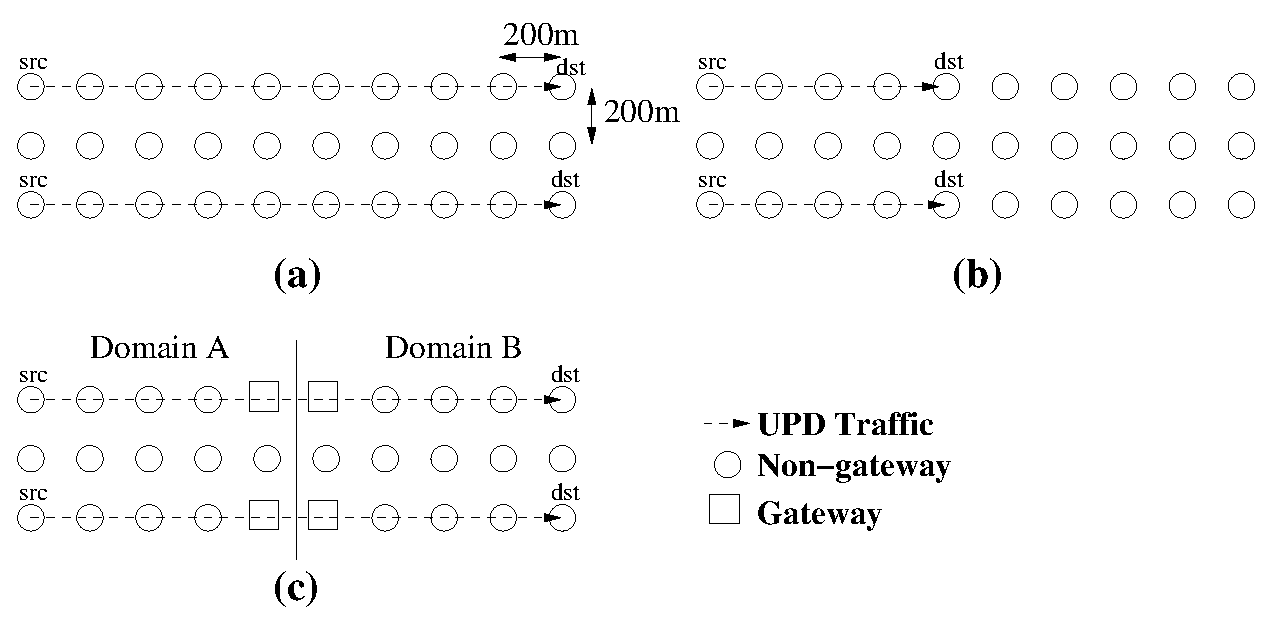
\includegraphics[width=0.47\textwidth]{figs/case1topo.eps}
\caption{Stationary grid topology for: (a) DSDV, and (b) IDRM} 
\label{fig:case1topo}
\end{figure}

We first study the performance of IDRM with
stationary grid topology shown in figure
\ref{fig:case1topo}. 
The goal here is to demostrate the performance of IDRM with multiple domains is
comparable to the performance of the single routing protocol with a signle domain.

We study the performance of IDRM in 3 different settings.
For all 3 cases, there are 2 UDP traffics.
In the first case (figure \ref{fig:case1topo}a), 
the src and the dst of each traffic are separated by 9 hops in a single DSDV domain.
In the second case (figure \ref{fig:case1topo}b), 
the setting is similar to figure \ref{fig:case1topo}a excepts
the src and the dst are separated by 4 hops.
In the last setting (figure \ref{fig:case1topo}c), 
the src and the dst are separated by 9 hops, and they are located in different DSDV domains.

Notice that in figure \ref{fig:case1topo}a and 
figure \ref{fig:case1topo}b, 
all nodes are communicate through one channel, 
while in figure \ref{fig:case1topo}c, 
nodes are using 3 independent channels 
(one for domain A, one for IDRM, and one for domain B). 

\begin{figure}[htb!] 
\center
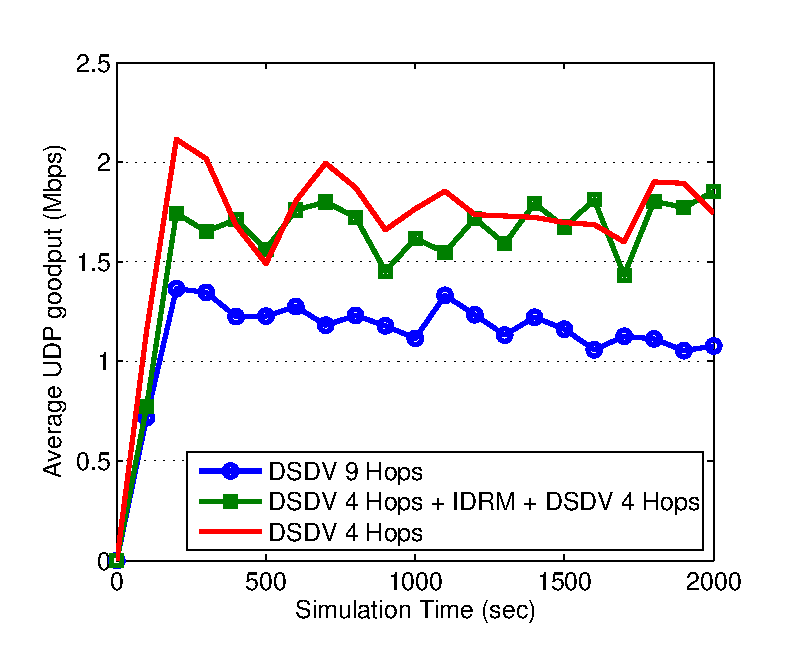
\includegraphics[width=0.47\textwidth, height=2.0in]{figs/case1DSDV.eps}
\caption{Aggregate UDP goodput for scenario 1}
\label{fig:case1udp}
\end{figure}

\begin{table}[htb!]
\center
\begin{tabular}{|c||c|c|c|c|}
\hline
 & IDRM & DSDV & Avgerage & Average\\
 & control pkts & control pkts & UDP goodput & E2E delay \\
\hline
DSDV 9 hops & N/A & 7353 & 1.115 Mbps &\\
\hline
DSDV 4 hops & N/A & 6891 & 1.547 Mbps &\\
\hline
IDRM + DSDV & 6309 & 5316 & 1.669 Mbps &\\
\hline
\end{tabular}
\caption{No. of control packets and average end-to-end delay}
\label{table:case1overhead}
\end{table}

The aggregate UDP goodput for all 3 cases are shown in figure \ref{fig:case1udp}.
IDRM with DSDV case performs better than DSDV 9 hops case because 
there are three independent channels, so the number of packet loss due to collision is less.


\subsection{Scenario 2: 2-domain topology with simple group mobility}
\label{sec:case2}

\begin{figure}[htb!] 
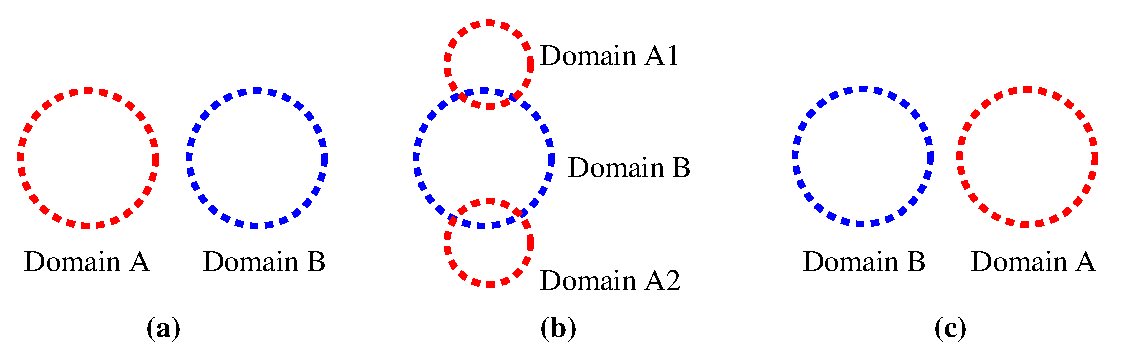
\includegraphics[width=0.47\textwidth]{figs/case2topo.eps}
\caption{Relative position of domain A and B at (a) Initial, (b) domain $A$
is partitioned, and (c) domain $A1$ and $A2$ are merged}
\label{fig:case2topo} 
\end{figure}

%we demostrate the changes of end-to-end
%performance with a simple scenario setting. 
%More detail study of random scenario will be shown in section \ref{sec:case3}.   
In this section, 
we study the performance of a simple group mobililty with 
2-domain topology shown in figure \ref{fig:case2topo}.
There are two domains in this scenario, namely domain $A$ and domain $B$. 
We create a synthetic group mobility for domain $A$ as follow: 
1) Initially, domain $A$ is located at the west side of domain $B$, 
2) After a while, domain $A$ is moving towards the east side of domain $B$ and
partitioned into two sub-domains $A1$ and $A2$,
3) Finally, $A1$ and $A2$ are merged back to domain $A$ and domain $A$ is
located at the east side of domain $B$. 
Two UDP traffics, $U1$ and $U2$, are created for the evaluation.
$U1$ is a traffic where the source is located in domain $A1$ and the destination
is located at domain $A2$. 
During domain $A$ is partitioned, $U1$ need to use the
path $A1\to B\to A2$ to maintain connectivity.
For $U2$, the source is located at domain $A$ and the destination is located at
domain $B$.


\subsection{Scenario 3: Random Topology}
\label{sec:case3}
In the previous examples, we illustrate the effectiveness of IDRM
with two simple scenarios. 
In this sections, we consider a more complex scenario with 
random topology. 
We randomly deployed 60 nodes in a 1000x1000 $m^{2}$ area,
and the random waypoint mobility mode is used.
Two average speed settings, 1.34m/s and 13.4m/s, 
are used to simulate walking and driving speed.
Also, we study the performance of IDRM with different percentage of
gateways and different number of domains.




%\subsubsection{}
%\begin{itemize}
%\item Correctness of IDRM:\\
%We validate the performance of IDRM. We use two grid network topologies for
%the verification: one is IDRM based heterogeneous MANETs and the other one is
%pure Ad-Hoc Routing Protocol based homogeneous MANET. Both topologies are
%identity excepting that IDRM based topology is composed of heterogeneous
%multiple domains. If the performance of IDRM with multiple domain topology is
%comparable to the performance of the pure routing protocol with a signle
%domain one, we assume that IDRM performs well. We measure UDP throughput for
%the comparison.\\ \emph{Expected Results}: IDRM shows the similar UDP
%throughout to DSDV/AODV.

%\item Functionality verification:\\
%We verify the functionalities of IDRM. We examine the success of packet
%delivery across domains. We use a domain partition and convergence scenario
%with simple group mobility. We have two domains named A and B, and two UDP
%traffics U1, U2 which are within domain A and across domains between A and B
%respectively. By the predefined group mobility, domain A is partitioned into
%two sub-domains, A1 and A2 and they are merged into domain A. Packets of U2
%are delivered across A and B and under domain partition, packets of U1 are
%delivered through A1, B, and A2. We evaluate UDP throughput of two traffics as
%nodes move.\\ \emph{Expected Results}: IDRM performs well under domain
%partition/convergence and overlap(partial overlap, full overlap)
%\end{itemize}

\subsection{Performance Metrics}
\emph{For each scenario, we will study the following metrics. 
So the following will be merged into the above 3 scenarios}\\
%\emph{After verifying the correctness and functionality of IDRM, we evaluate
%the performance of IDRM on large scale network topology.}\\

\subsubsection{Network Reachability}
We measure the network reachablity with different control parameters.
We quantify the network reachability as the number of nodes that each node can reach at a moment.
We assume the more number of reachable nodes means the better network reschability.
We control the number of gateways and the interval of control packets.
\begin{itemize}
\item x-axis: time, or different parameters
\item y-axis: Average number of reachable node for each node
\item \emph{Expected Results}: Each gateway is able to logically reach to all of nods physically reachable through other gateways.\\
\end{itemize}

\subsubsection{Route Convergence}
We measure the delay of route update messages over the entire network.
The delay starts when a route update message is generated by a node and ends when every gateway reachable to the node receives the update message.
We control the interval of control messages, communication range, and mobility for the evaluation.

\begin{itemize}
\item x-axis: Beacon interval time, different node speed and communication range
\item y-asix: Average Route Convergence time\\
\end{itemize}

\subsubsection{Route Consistence}
We define a consistent route as a route entry that every gateway reachable to the entry has the same status of the entry.
Because of network dynamics, it is possible that some of gateways have a valid value to the invalid entries.
We control the interval of control messages, communication range, and mobility for the evaluation.
As we have the global information in ns2, [Difficult to do] present the % of route entry in IDRM route tables which contains inconsistence values.

\subsubsection{UDP Throughput and Delay}
We randomly generate disjoint source and destination pairs of UDP traffics and measure the throughput,
and end-to-end delay of the traffics under network dynamics.

\begin{itemize}
\item x-axis: time, series: different parameters
\item y-axis: UDP throughput, end-to-end delay\\
\end{itemize}

\subsubsection{Overhead}
We define the overhead of IDRM as the number of/ and the amount of IDRM control packets.
We plot the percentage of each type of packets: data, IDRM packets.\\
\begin{itemize}
\item \emph{Expected Results}: As tested with a small topology(two domains, 6 nodes), the overhead of IDRM was less than 2\% and rest of packets were data.
\end{itemize}
